%--------------------------------------------------------------------------------
%
%
%--------------------------------------------------------------------------------
\chapter*{Stack Layout}
\addcontentsline{toc}{chapter}{Stack Layout}

Note: sketches and notes for now...

\section*{Stack Frame}
\addcontentsline{toc}{section}{Stack Frame Marker}

\section*{Stack Frame Marker}
\addcontentsline{toc}{section}{Stack Frame Marker}

stack frame marker has four double words. ( make it a picture ... )

\begin{figure}[H]
\begin{center}
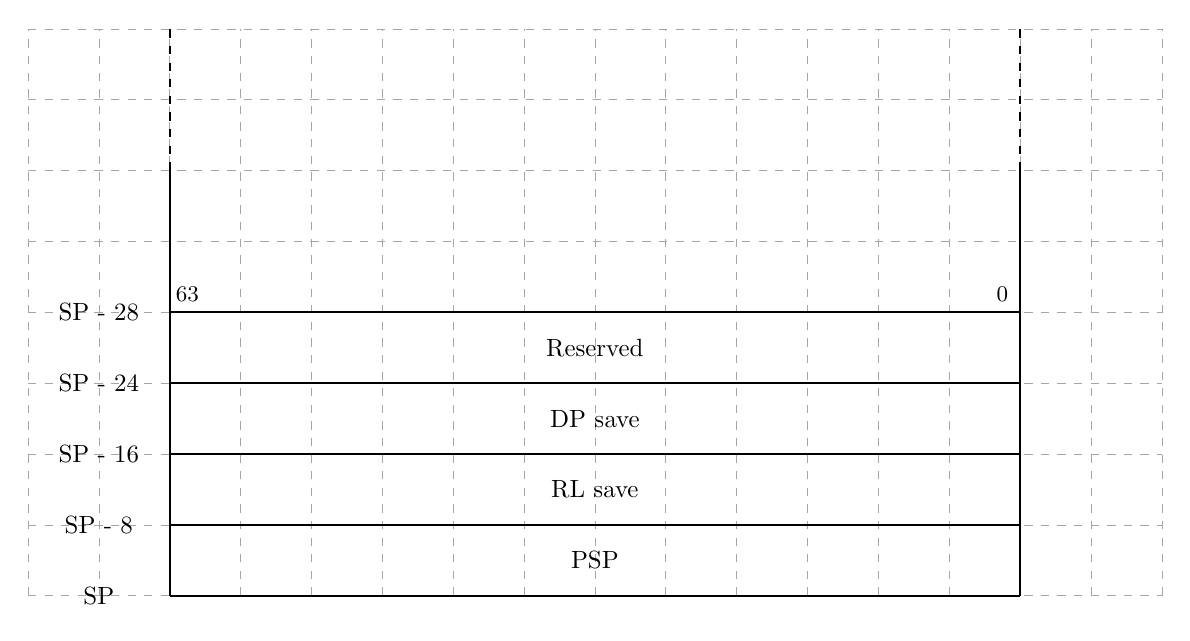
\begin{tikzpicture}[scale=0.9, transform shape]
        
  	\draw[help lines, gray!70, dashed] (0,0) grid(16,8);
  	
  	% Rectangle dimensions
	\def\width{12}
	\def\leftofs{2}
	\def\rightofs{\leftofs + \width}
  	\def\middleofs{ \leftofs + \width / 2 }
  	
  	% Bits
  	\node at (\leftofs + 0.25,4 + 0.25) {\small 63};
	\node at (\rightofs - 0.25,4 + 0.25) {\small 0};

	% Box
	\draw[thick] (\leftofs, 0) -- (\leftofs, 4);
	\draw[thick] (\rightofs, 0) -- (\rightofs, 4);
	\draw[thick] (\leftofs, 0) -- (\rightofs, 0);
	\draw[thick] (\leftofs, 4) -- (\rightofs, 4);
	
	\draw[thick] (\leftofs, 4) -- (\leftofs, 6);
	\draw[thick, dashed] (\leftofs, 6) -- (\leftofs, 8);
	
	\draw[thick] (\rightofs, 4) -- (\rightofs, 6);
	\draw[thick, dashed] (\rightofs, 6) -- (\rightofs, 8);
	
	\node at ({\leftofs - 1}, {4}) { SP - 28 };

	% Fields 
	% reserved
	\draw[thick] (\leftofs, 3) -- (\rightofs, 3);
  	\node at ({\leftofs - 1}, {3}) { SP - 24 };
  	\node at ( \middleofs, {3 + 0.5}) { Reserved};	
  	
  	% DP Save
  	\draw[thick] (\leftofs, 2) -- (\rightofs, 2);
  	\node at ({\leftofs - 1}, {2}) { SP - 16 };
  	\node at ( \middleofs, {2 + 0.5}) { DP save};
  	
  	% RL Save
  	\draw[thick] (\leftofs, 1) -- (\rightofs, 1);
  	\node at ({\leftofs - 1}, {1}) { SP - 8 };
  	\node at ( \middleofs, {1 + 0.5}) { RL save };
  	
  	% PSP
  	\draw[thick] (\leftofs, 0) -- (\rightofs, 0);
  	\node at ({\leftofs - 1}, {0}) { SP };
  	\node at ( \middleofs, {0 + 0.5}) { PSP };
  
\end{tikzpicture}
\end{center}
\caption{Stack Frame Marker}
\label{fig:Stack Frame Marker}
\end{figure}


A stack frame marker could also be smaller, if we consider to put DP and the reserved word as local variables in the stack frame.
